%=================================================
% Economics Coursework Template
%=================================================
\documentclass[12pt]{article}

%------------ Packages ------------
\usepackage[margin=1in]{geometry}   % Page layout
\usepackage{lmodern}                % Latin Modern (LaTeX default font)
\usepackage{amsmath, amssymb}       % Math symbols
\usepackage{booktabs}               % Professional tables
\usepackage{graphicx}               % Figures
\usepackage{natbib}                 % References
\usepackage[hidelinks]{hyperref}    % Hyperlinks
\usepackage{fancyhdr}               % Headers/footers
\usepackage{setspace}               % Line spacing
\usepackage{titlesec}               % Section formatting
\usepackage{comment} 
\usepackage{xcolor} 
\usepackage{amsthm} 
\usepackage{float} 
\usepackage{dcolumn}
\usepackage{tikz}
\usetikzlibrary{arrows.meta,positioning,fit,calc}
\tikzset{
  var/.style={rectangle, draw, rounded corners, minimum width=18mm, minimum height=7mm, align=center},
  latent/.style={ellipse, draw, dashed, minimum width=18mm, minimum height=7mm, align=center},
  controlarrow/.style={->, dashed, draw=red!60},
  lightbluearrow/.style={->, dashed, draw=blue!40} % NEW style
}

%------------ Page Style ------------
\rhead{\thepage}
\lhead{ECO1465 Weekly Report 1}

%------------ Section Formatting ------------
\titleformat{\section}{\large\bfseries}{\thesection.}{0.5em}{}
\titleformat{\subsection}{\normalsize\bfseries\itshape}{\thesubsection}{0.5em}{}
\titlespacing*{\subsection}{0pt}{1.5ex plus 1ex minus .2ex}{1em} % spacing before/after subsections


%------------ Begin Document ------------
\begin{document}
% Title Page only
\begin{titlepage}
    \thispagestyle{empty} % no headers/footers
    \centering
    \vspace*{\fill}

    {\Large \textbf{Double Machine Learning} \par}
    \vspace{0.5em}
    {\normalsize Applied Causal Machine Learning \par}
    {\normalsize Week 12 Report \par}

    \vspace{3em}
    {\large Nardeen Abdulkareem -- 1009722089 \par}
    {\normalsize The University of Toronto \par}
    {\normalsize \today \par}
    {\texttt{nardeen.abdulkareem@mail.utoronto.ca} \par}

    \vspace*{\fill}
\end{titlepage}
\clearpage

\section{Paper Title}
Who gets left behind? Do Woman Disproportionally Benefits from the Jóvenes en Acción Vocational Training Program?

\section{One-Paragraph Research Summary}

This study investigates why women experience disproportionately larger gains in employment outcomes than men following participation in the Jóvenes en Acción vocational training program in Colombia. The analysis uses publicly available individual-level data from the randomized controlled trial conducted by Attanasio, Kugler, and Meghir (2011), which follows 3,215 participants—1,693 treated and 1,759 women—across Colombia’s seven largest cities. The data combine baseline and follow-up survey information on demographic, educational, and labor-market characteristics. The outcome variables are (i) employment status, (ii) paid employment, and (iii) annual real salary, each measured two years after program completion. The key variables of interest are treatment assignment (program participation), gender, and their interaction term (Treatment × Female), with pre-treatment controls including education level, age, marital status, and prior employment indicators. The research aims to uncover the mechanisms driving gender-differentiated treatment effects and to identify how pre-existing labor-market attachment and geographic context shape post-program outcomes.

\section{Linear Double Machine Learning Model}
The treatment variable is program selection, and the outcome is employment in 2006 (empl\_06). After training the linear DML model, I obtain the individual conditional average treatment effects (CATEs) and compute the average treatment effect (ATE): 0.022 with a 95\% CI of $(0.015, 0.030)$.

\section{Non-Linear DML}
Next, I estimate a non-linear Double ML model using a Causal Forest. This model relaxes the linearity assumptions and allows treatment effects to vary flexibly and interact with covariates in arbitrary ways. This is useful if the effect of the program differs across demographic groups, education levels, or prior labour market characteristics. The resulting ATE from the causal forest is: 0.022 with a 95\% CI of(0.019, 0.026). The confidence interval is narrower which is good for inference. However, surprisingly, the non-linear model produces an ATE almost identical to the linear model. We can also attain this CATE estimate for being a women ATE (women): 0.040. ATE (men): 0.002. This is statistically significant, the ATE using DML is similar to the one we attained from Doubly Robust Learners, and the heterogeneity for the women indicator is nearly identical to that of the Causal Forest (obviously).

\section{Cumulative Gain Plots}
\begin{figure}[H]
    \centering
    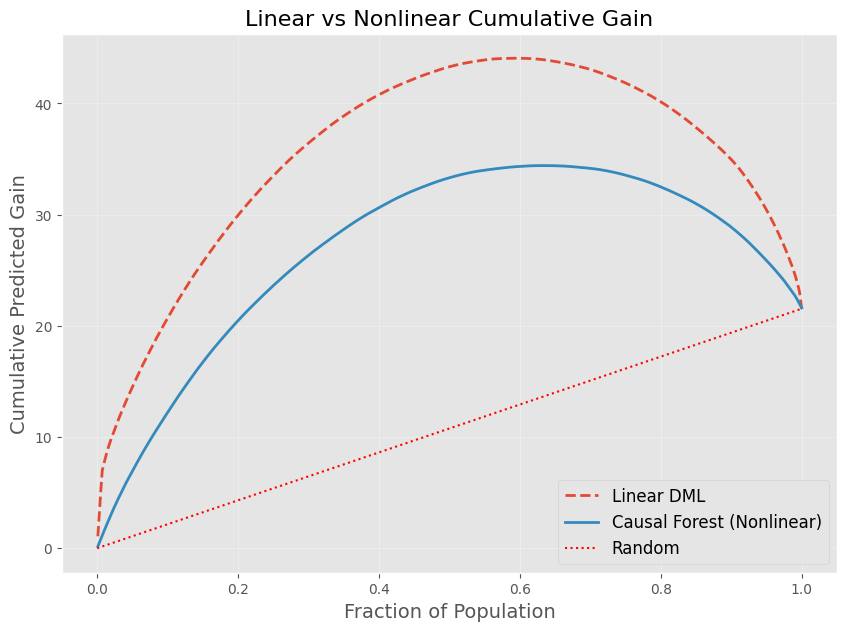
\includegraphics[scale=0.7]{1.png} 
    \caption{Cumulative Gain Plot}
\end{figure}

Both models outperform random assignment. The linear model (red dashed line) reaches a peak cumulative gain of roughly 45, outperforming the non-linear model. When individuals are ranked by predicted treatment effect, the linear model identifies the highest-gain participants more sharply. 

Causal forest curve is smoother and more conservative. This is due to regularization in the forest estimator and the models tendency to avoid extreme predictions unless strongly justified by the data. The ATEs are nearly identical, meaning the models generally agree in results. But the ranking of individuals by treatment effect differs, which is what the cumulative gain curves capture.

The linear model is more aggressive and assigns larger positive and negative effects, producing a steeper uplift curve. The non-linear model is more cautious, distributing treatment effects more conservatively.



\end{document}


